\documentclass[a4paper,10pt,bg=full]{dndbook} %a4, 10pt, bg=print / full
\usepackage[english]{babel} %language
\usepackage[utf8]{inputenc} %lovely utf-8
\usepackage{graphicx} %images
\usepackage{array} %allways use this shit, idk why
\usepackage{tikz} %draw stuff
\usepackage{ifthen} %draw stuff
\usetikzlibrary{calc,fadings} %draw stuff
\usepackage{xspace} %usefull idk, allways import this stuff
\usepackage{setspace} %don't ask, kind of like it...
\usepackage{pgfplots}
\usepackage{tabularx} % table
\usepackage[singlelinecheck=false]{caption} %idk dndbook...
\usepackage{listings} %idk dndbook...
\usepackage{stfloats} %idk dndbook
\usepackage{yfonts}
\usepackage{aurical}
\usepackage[T1]{fontenc}

\graphicspath{ {./images/} }

\pagestyle{empty} % no footer

\geometry { % paper type + spacing
	a4paper,
	top=2cm,
	bottom=2cm,
	left=2cm,
	right=2cm
}
\newcommand*\circled[2][2pt]{
	\tikz
	[
		decoration={
			random steps,
			amplitude=1pt,
			segment length=5pt
		},
		baseline=(char.base)
	]{
		\node
		[
			decorate,
			shape=circle,
			draw,
			inner sep=#1-1pt
		]
		(char) {#2};
	}
}

\singlespacing
\makeatletter

\def \license {GNU Free Documentation License (https://www.gnu.org/licenses/fdl-1.3)}
\def \author {Sven Hugi}%if you edit this document, add your name... <3

%highlighting with some random effect -> looks handmade and i love it... you can use this in you texts
\newcommand\hl[2][yellow]{
	\begin{tikzpicture}[
	baseline,
	decoration={random steps,amplitude=1pt,segment length=15pt},
	outer sep=-15pt, inner sep = 0pt
	]
	\node[decorate,rectangle,fill=#1,anchor=text]{#2\xspace};
	\end{tikzpicture}
}
% colors:

% bgtan
% bgtan2018
% pagegold

% titlered
% titlegold
% rulered
% contourgray

% BrGreen
% PhbLightGreen
% PhbLightCyan
% PhbMauve
% PhbTan
% DmgLavender
% DmgCoral
% DmgSlateGray
% DmgLilac

%config:
\def\Name{}
\def\offset{-5.67} % change, if the line at the top is staggered -> -5.67 is the default value -> should work in ~100% of the cases

\def\CharaClass{}
\def\Level{}
\def\Background{}
\def\Playername{}
\def\Race{}
\def\Alignment{}
\def\EP{}

\def\Speed{}
\def\Initiative{}
\def\AC{}
\def\Prof{}

\def\MaxHP{}
\def\HitDice{}

\def\Str{}
\def\Dex{}
\def\Con{}
\def\Int{}
\def\Wis{}
\def\Cha{}

\def\StrMod{}
\def\DexMod{}
\def\ConMod{}
\def\IntMod{}
\def\WisMod{}
\def\ChaMod{}

\def\StrSave{}
\def\DexSave{}
\def\ConSave{}
\def\IntSave{}
\def\WisSave{}
\def\ChaSave{}

% save profs
\def\firstStat{}
\def\secondStat{}

% modifiers for skills (add prof bonus if prof)
%str
\def\Athletics{}
%dex
\def\Acrobatics{}
\def\SleightOfHand{}
\def\Stealth{}
%int
\def\Arcana{}
\def\History{}
\def\Investigation{}
\def\Nature{}
\def\Religion{}
%wis
\def\AnimalHandling{}
\def\Insight{}
\def\Medicine{}
\def\Perception{}
\def\Survival{}
%cha
\def\Deception{}
\def\Intimidation{}
\def\Performance{}
\def\Persuasion{}

% prof (0/1)
\def\AthleticsProf{0}
%dex
\def\AcrobaticsProf{0}
\def\SleightOfHandProf{0}
\def\StealthProf{0}
%int
\def\ArcanaProf{0}
\def\HistoryProf{0}
\def\InvestigationProf{0}
\def\NatureProf{0}
\def\ReligionProf{0}
%wis
\def\AnimalHandlingProf{0}
\def\InsightProf{0}
\def\MedicineProf{0}
\def\PerceptionProf{0}
\def\SurvivalProf{0}
%cha
\def\DeceptionProf{0}
\def\IntimidationProf{0}
\def\PerformanceProf{0}
\def\PersuasionProf{0}

\def\Age{}
\def\Height{}
\def\Weight{}
\def\Skin{}
\def\Eyes{}
\def\Hair{}

\def\SpellAbility{}
\def\SpellAtk{}
\def\SpellSaveDC{}

\def\FirstLevelSlots{}
\def\SecondLevelSlots{}
\def\ThirdLevelSlots{}
\def\FourthLevelSlots{}
\def\FifthLevelSlots{}
\def\SixthLevelSlots{}
\def\SeventhLevelSlots{}
\def\EightLevelSlots{}
\def\NinthLevelSlots{}

\def\Cantrips{
	%\small %uncomment for non-wizards...
	\begin{tabularx}{\linewidth}{lX}
	%	\textbf{Mage Hand} & Usefull cantrip, because usefull\\%Example
	\end{tabularx}
}
\def\FirstLevelSpells{
	\begin{tabularx}{\linewidth}{lX}
		
	\end{tabularx}
}
\def\SecondLevelSpells{
	\begin{tabularx}{\linewidth}{lX}
		
	\end{tabularx}
}
\def\ThirdLevelSpells{
	%\small %uncomment for non-wizards...
	\begin{tabularx}{\linewidth}{lX}
		
	\end{tabularx}
}
\def\FourthLevelSpells{
	\begin{tabularx}{\linewidth}{lX}
		
	\end{tabularx}
}
\def\FifthLevelSpells{
	\begin{tabularx}{\linewidth}{lX}
		
	\end{tabularx}
}
\def\SixthLevelSpells{
	%\small %uncomment for non-wizards...
	\begin{tabularx}{\linewidth}{lX}
		
	\end{tabularx}
}
\def\SeventhLevelSpells{
	\begin{tabularx}{\linewidth}{lX}
		
	\end{tabularx}
}
\def\EightLevelSpells{
	\begin{tabularx}{\linewidth}{lX}
		
	\end{tabularx}
}
\def\NinthLevelSpells{
	\begin{tabularx}{\linewidth}{lX}
		
	\end{tabularx}
}

\def\Description{
}

\def\WeaponEquipment{
	%max 4 weapons -> with some only 3, with morningstar & co 5
		%Example (uncomment to test):
		%\textbf{Shortsword}\\
		%\raggedleft
		%+10 1d6 + 4 Piercing\\
		%Light, Finesse\\
		%\raggedright
}

\def\WeaponProf{
	%warning, empty itemize throws error -> empty item placed -> don't let this unused...
	\begin{itemize}
	%	\item[$\bullet$] Longsword % Example
	\item
	\end{itemize}
}
\def\ArmorProf{
	\begin{itemize}
	%	\item[$\bullet$] Light Armor %Example
	\item
	\end{itemize}
}
\def\LanguageProf{
	\begin{itemize}
	%	\item[$\bullet$] Common %Example
	\item
	\end{itemize}
}
\def\ToolProf{
	\begin{itemize}
	%	\item[$\bullet$] Smith’s tools %Example
	\item
	\end{itemize}
}

\def\ClassFeature{
	\begin{tabularx}{\textwidth}{lX}
	%	\textbf{Spellcasting}	& You have a spellbook containing spells.\\ %Example
	\end{tabularx}
}
\def\RaceFeature{
	\begin{tabularx}{\textwidth}{lX}
		%\textbf{Darkvision}	& 60ft dim Light see as bright, darkness as dim. No color in darkness.\\ %Example
		%\textbf{Darkvision}	& 60ft\\ %other example
	\end{tabularx}
}
\def\BackgroundFeature{
	\begin{tabularx}{\textwidth}{lX}
	%	\textbf{All Eyes on You}	& You can parley attention into access to people and places.\\ %Example
	\end{tabularx}
}

%static -> don't use for changing stuff, like arows, food etc
\def\Equipment{
	\begin{tabularx}{\textwidth}{lX}
		%\textbf{Rope}	& $50ft$ % Example
	\end{tabularx}
}

%%%%%%%%%%%%%%%%%%%%%%%%%%%%%%%%%Document%%%%%%%%%%%%%%%%%%%%%%%%%%%%%%%%%
\begin{document}
	\begin{minipage}[t]{.5\linewidth} % head left
		\begin{tabularx}{\textwidth}{XXX}
			\multicolumn{3}{X}{\Fontauri\Name}\\\hline
			\multicolumn{3}{X}{\tiny{Character Name}}\\
			\AC & \Initiative & \Speed {\small$^{ft}$}\\\hline
			\tiny{AC}&\tiny{Initiative}&\tiny{Speed}\\
			\HitDice&\Level&\\\hline
			\tiny{Hit Dice}&\tiny{Total}&\tiny{Used}\\
			\MaxHP&&\\\hline
			\tiny{Max Hp}&\tiny{Hp}&\tiny{Temp Hp}\\
			\Prof&&\\\hline
			\tiny{Proficiency Bonus}
		\end{tabularx}
	\end{minipage}%
	\begin{minipage}[t]{.5\linewidth} % head right
		\strut\vspace*{\offset\baselineskip}\newline %correct offset because of a fontsize and b minipage
		\begin{tabularx}{\textwidth}{XXX}
			\CharaClass\space\Level &\Background &\Playername\\\hline
			\tiny{Class \& Level}	& \tiny{Background}	&\tiny{Player Name}\\
			\Race &\Alignment &\EP\\\hline
			\tiny{Race}	& \tiny{Alignment}	&\tiny{EP}\\
		\end{tabularx}\vspace*{.125cm}\\
		\Fontauri\large{
			\begin{tabularx}{\linewidth}{XXXXXX}
				Str & Dex & Con & Int & Wis & Cha \\ \hline
				\Str & \Dex & \Con & \Int & \Wis & \Cha\\
				\ifthenelse{\equal{\firstStat}{Str}}{$\bullet$}{\ifthenelse{\equal{\secondStat}{Str}}{$\bullet$}{}} &
				\ifthenelse{\equal{\firstStat}{Dex}}{$\bullet$}{\ifthenelse{\equal{\secondStat}{Dex}}{$\bullet$}{}} &
				\ifthenelse{\equal{\firstStat}{Con}}{$\bullet$}{\ifthenelse{\equal{\secondStat}{Con}}{$\bullet$}{}} &
				\ifthenelse{\equal{\firstStat}{Int}}{$\bullet$}{\ifthenelse{\equal{\secondStat}{Int}}{$\bullet$}{}} &
				\ifthenelse{\equal{\firstStat}{Wis}}{$\bullet$}{\ifthenelse{\equal{\secondStat}{Wis}}{$\bullet$}{}} &
				\ifthenelse{\equal{\firstStat}{Cha}}{$\bullet$}{\ifthenelse{\equal{\secondStat}{Cha}}{$\bullet$}{}}\\
				\StrMod & \DexMod & \ConMod & \IntMod & \WisMod & \ChaMod\\
				\StrSave & \DexSave & \ConSave & \IntSave & \WisSave & \ChaSave
			\end{tabularx}
	}
	\end{minipage}\vspace*{.25cm}\\
	\begin{minipage}[t]{.25\linewidth}\normalsize
		{\LARGE Skills}\\
		\textcolor{titlered}{\large Strength \StrMod \ifthenelse{\equal{\firstStat}{Str}}{$\bullet$}{\ifthenelse{\equal{\secondStat}{Str}}{$\bullet$}{}}}\\
		\begin{tabularx}{\textwidth}{lXr}
			\ifthenelse{\equal{\AthleticsProf}{1}}{$\bullet$}{}&Athletics&\Athletics\\
		\end{tabularx}
		\textcolor{titlered}{\large Constitution \ConMod \ifthenelse{\equal{\firstStat}{Con}}{$\bullet$}{\ifthenelse{\equal{\secondStat}{Con}}{$\bullet$}{}}}\\
		\textcolor{titlered}{\large Dexterity \DexMod \ifthenelse{\equal{\firstStat}{Dex}}{$\bullet$}{\ifthenelse{\equal{\secondStat}{Dex}}{$\bullet$}{}}}\\
		\begin{tabularx}{\textwidth}{lXr}
			\ifthenelse{\equal{\AcrobaticsProf}{1}}{$\bullet$}{}&Acrobatics&\Acrobatics\\
			\ifthenelse{\equal{\SleightOfHandProf}{1}}{$\bullet$}{}&Sleight of Hand&\SleightOfHand\\
			\ifthenelse{\equal{\StealthProf}{1}}{$\bullet$}{}&Stealth&\Stealth\\
		\end{tabularx}
		\textcolor{titlered}{\large Intelligence \IntMod \ifthenelse{\equal{\firstStat}{Int}}{$\bullet$}{\ifthenelse{\equal{\secondStat}{Int}}{$\bullet$}{}}}\\
		\begin{tabularx}{\textwidth}{lXr}
			\ifthenelse{\equal{\ArcanaProf}{1}}{$\bullet$}{}&Arcana&\Arcana\\
			\ifthenelse{\equal{\HistoryProf}{1}}{$\bullet$}{}&History&\History\\
			\ifthenelse{\equal{\InvestigationProf}{1}}{$\bullet$}{}&Investigation&\Investigation\\
			\ifthenelse{\equal{\NatureProf}{1}}{$\bullet$}{}&Nature&\Nature\\
			\ifthenelse{\equal{\ReligionProf}{1}}{$\bullet$}{}&Religion&\Religion\\
		\end{tabularx}
		\textcolor{titlered}{\large Wisdom \WisMod \ifthenelse{\equal{\firstStat}{Wis}}{$\bullet$}{\ifthenelse{\equal{\secondStat}{Wis}}{$\bullet$}{}}}\\
		\begin{tabularx}{\textwidth}{lXr}
			\ifthenelse{\equal{\AnimalHandlingProf}{1}}{$\bullet$}{}&Animal Handling&\AnimalHandling\\
			\ifthenelse{\equal{\InsightProf}{1}}{$\bullet$}{}&Insight&\Insight\\
			\ifthenelse{\equal{\MedicineProf}{1}}{$\bullet$}{}&Medicine&\Medicine\\
			\ifthenelse{\equal{\PerceptionProf}{1}}{$\bullet$}{}&Perception&\Perception\\
			\ifthenelse{\equal{\SurvivalProf}{1}}{$\bullet$}{}&Survival&\Survival\\
		\end{tabularx}
		\textcolor{titlered}{\large Charisma \ChaMod \ifthenelse{\equal{\firstStat}{Cha}}{$\bullet$}{\ifthenelse{\equal{\secondStat}{Cha}}{$\bullet$}{}}}\\
		\begin{tabularx}{\textwidth}{lXr}
    		\ifthenelse{\equal{\DeceptionProf}{1}}{$\bullet$}{}&Deception&\Deception\\
			\ifthenelse{\equal{\IntimidationProf}{1}}{$\bullet$}{}&Intimidation&\Intimidation\\
			\ifthenelse{\equal{\PerformanceProf}{1}}{$\bullet$}{}&Performance&\Performance\\
			\ifthenelse{\equal{\PersuasionProf}{1}}{$\bullet$}{}&Persuasion&\Persuasion\\
		\end{tabularx}
		\textcolor{titlered}{\large Weapons}\linebreak
		\WeaponEquipment
	\end{minipage}%
	\begin{minipage}[t]{.25\linewidth}\normalsize
		{\LARGE Proficiencies}
		\textcolor{titlered}{\large Weapons}\\
		\WeaponProf
		\textcolor{titlered}{\large Armor}\\
		\ArmorProf
		\textcolor{titlered}{\large Language}\\
		\LanguageProf
		\textcolor{titlered}{\large Tools}\\
		\ToolProf
	\end{minipage}%
	\begin{minipage}[t]{.5\linewidth}\raggedleft\normalsize
		{\LARGE Features}\\
		\textcolor{titlered}{\large \Background}\\
		\BackgroundFeature
		\textcolor{titlered}{\large \Race}\\
		\RaceFeature
		\textcolor{titlered}{\large \CharaClass}\\
		\ClassFeature
	\end{minipage}\\
	\begin{minipage}[t][\textheight]{.5\linewidth}\normalsize
		{\LARGE Equipment}\\
		\Equipment
	\end{minipage}%
	\begin{minipage}[t][\textheight]{.5\linewidth}\normalsize
		\begin{tabularx}{\textwidth}{XXX}
			&&\\\hline
			\tiny{PP}&\tiny{GP}	&\tiny{EP}\\
			&&\\\hline
			\tiny{SP}& \tiny{CP}&
		\end{tabularx}\vspace*{.25cm}\\
		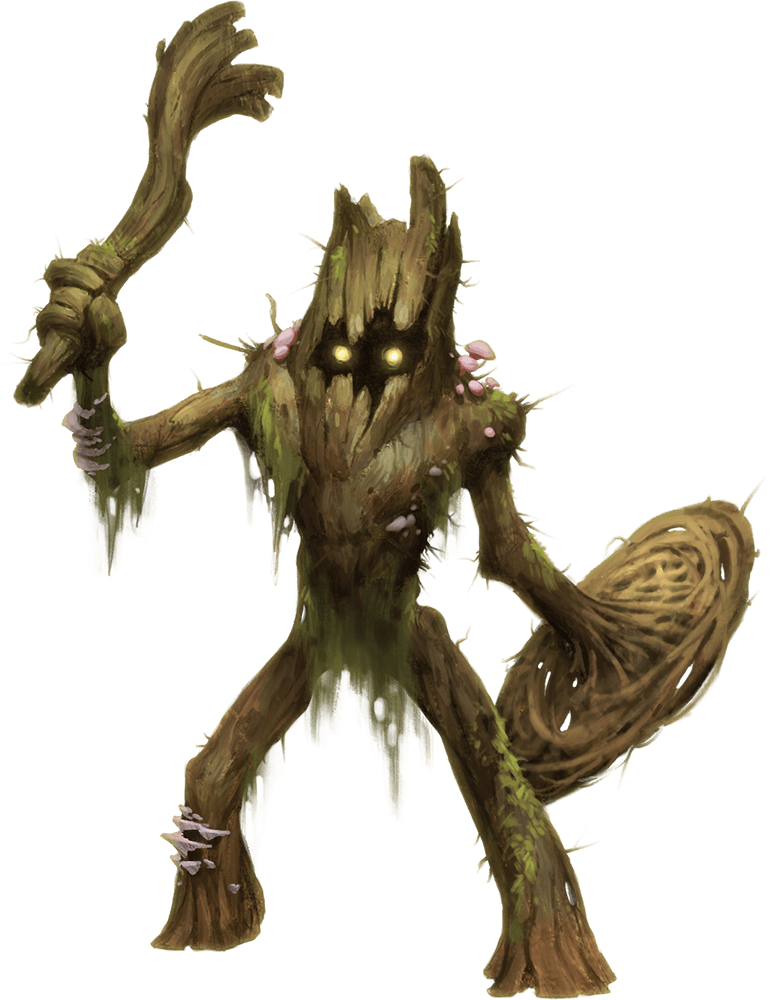
\includegraphics[width=\linewidth]{Character.png}\vspace*{.25cm}\\
		\begin{tabularx}{\textwidth}{XXX}
			\Age &\Height &\Weight\\\hline
			\tiny{Age}	& \tiny{Height}	&\tiny{Weight}\\
			\Eyes &\Skin &\Hair\\\hline
			\tiny{Eyes}	& \tiny{Skin}	&\tiny{Hair}\\
		\end{tabularx}
		{\LARGE Character Description}\\
		{\scriptsize\Description}
	\end{minipage} %
	{\huge Spellcasting}
	\begin{center}\normalsize
		\begin{tabularx}{\textwidth}{XXX}
			\SpellAbility &\SpellAtk &\SpellSaveDC\\\hline
			\tiny{Spellcasting Ability}	& \tiny{Spell Attack Bonus}	&\tiny{Spell Save DC}
		\end{tabularx}
		\begin{tabularx}{\linewidth}{XXXXXXXXX}
			1&2&3&4&5&6&7&8&9\\\hline
			\FirstLevelSlots&
			\SecondLevelSlots&
			\ThirdLevelSlots&
			\FourthLevelSlots&
			\FifthLevelSlots&
			\SixthLevelSlots&
			\SeventhLevelSlots&
			\EightLevelSlots&
			\NinthLevelSlots
		\end{tabularx}
	\end{center}
	\begin{minipage}[t]{.334\linewidth}\scriptsize
		\textcolor{titlered}{\large Cantrips}\\
		\Cantrips
		\textcolor{titlered}{\large 1st Level}\\
		\FirstLevelSpells
		\textcolor{titlered}{\large 2nd Level}\\
		\SecondLevelSpells
	\end{minipage}%
	\begin{minipage}[t]{.333\linewidth}\scriptsize
		\textcolor{titlered}{\large 3th Level}\\
		\ThirdLevelSpells
		\textcolor{titlered}{\large 4th Level}\\
		\FourthLevelSpells
		\textcolor{titlered}{\large 5th Level}\\
		\FifthLevelSpells
	\end{minipage}%
	\begin{minipage}[t]{.333\linewidth}\scriptsize
		\textcolor{titlered}{\large 6th Level}\\
		\SixthLevelSpells
		\textcolor{titlered}{\large 7th Level}\\
		\SeventhLevelSpells
		\textcolor{titlered}{\large 8th Level}\\
		\EightLevelSpells
		\textcolor{titlered}{\large 9th Level}\\
		\NinthLevelSpells
	\end{minipage} %
\end{document}